\documentclass{../source/Experiment}
\usepackage{subfig}

\major{信息工程}
\name{}
\title{OrCAD使用练习}
\stuid{}
\college{信息与电子工程学院}
\date{\today}
\lab{东4-216}
\course{电子电路设计实验}
\instructor{李锡华、施红军、叶险峰}
\grades{}
\expname{OrCAD使用练习}
\exptype{研究实验}
\partner{}

\begin{document}
    \makecover
    \makeheader

    \section{实验目的}
        \begin{enumerate}
            \item 了解OrCAD套件中的Capture和PSpiceA/D软件的基本菜单和命令的使用
            \item 掌握OrCAD中Capture软件的电路图输入和编辑方法
            \item 学习OrCAD中PSpiceA/D软件的分析设置、仿真、波形查看的方法。
            \item 学习半导体器件特性、电路特性的仿真分析方法
        \end{enumerate}
    
    \section{试验任务和要求}
        \subsection{实验任务}
            \begin{enumerate}
                \item 完成桥式整流电路(瞬态分析),查看输出波形情况
                \item 稳压二极管电路(瞬态分析),查看输出波形情况
            \end{enumerate}
        \subsection{实验要求}
            \begin{enumerate}
                \item 根据所给原理图设计简化实验电路。
                \item 根据设计电路设计并进行仿真实验。
                \item 根据仿真结果分析电路特性
            \end{enumerate}
            
    \section{实验方案设计与实验参数计算}
            \subsection{完整实验电路}
            \newpage
            \begin{figure}[h]          
                \begin{minipage}[t]{0.5\textwidth}
                    \centering
                    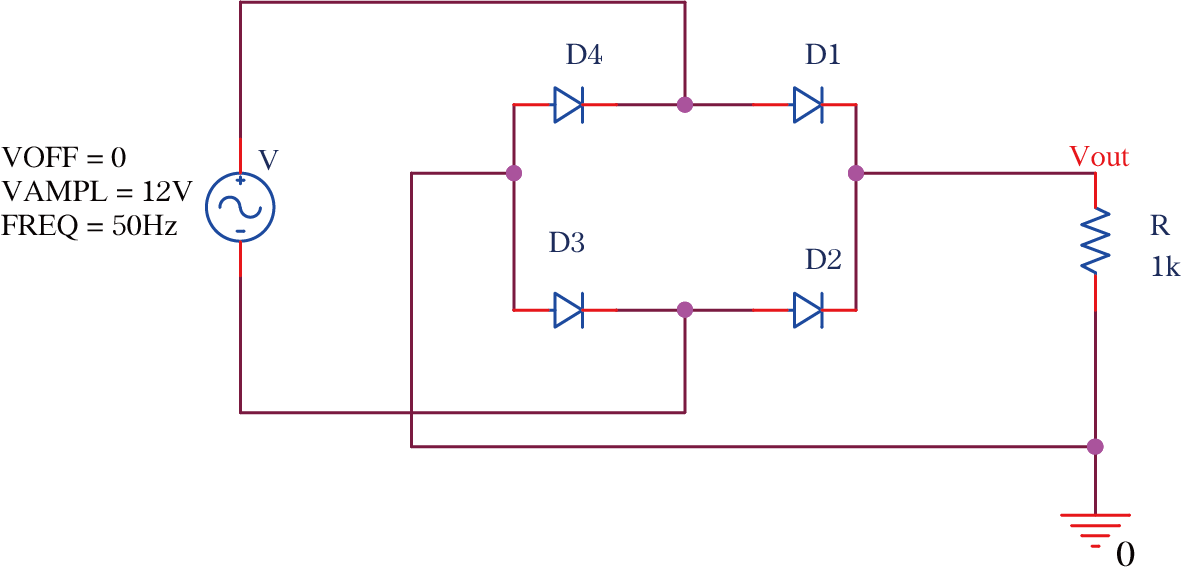
\includegraphics[scale=0.8]{pic/桥式与稳压二极管/brg1.png}
                    \caption{桥式整流电路\label{fig:1}}
                \end{minipage}
                \qquad
                \begin{minipage}[t]{0.5\textwidth}
                    \centering
                    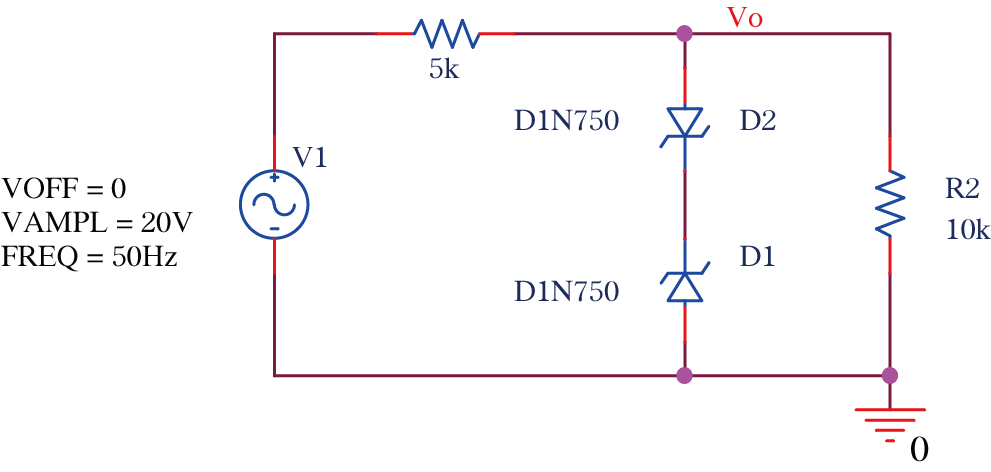
\includegraphics[scale=0.8]{pic/桥式与稳压二极管/d1.png}
                    \caption{稳压二极管\label{fig:2}}
                \end{minipage}
            \end{figure}
            \subsection{实验总体方案设计}
            \begin{enumerate}
                \item 根据原理图简化设计出电路图,并连接好电路。
                \item 根据电源以及元件调整合适的仿真分析参数,选择合适的仿真分析模式,进行仿真。
                \item 进行仿真实验,分析波形。
            \end{enumerate}

    \section{主要仪器设备}
            电脑,$OrCAD$软件

    \section{实验步骤、实验调试过程、实验数据记录}
            \subsection{实验步骤}
                \subsubsection{桥式整流电路分析}
                    \begin{enumerate}
                        \item 在$OrCAD$软件中按照图1连接好电路。
                        \item 根据电路电源的参数以及实验要求选择合适的仿真模式与参数。具体见下图。
                        \newpage
                        \begin{figure}[h]
                            \centering
                            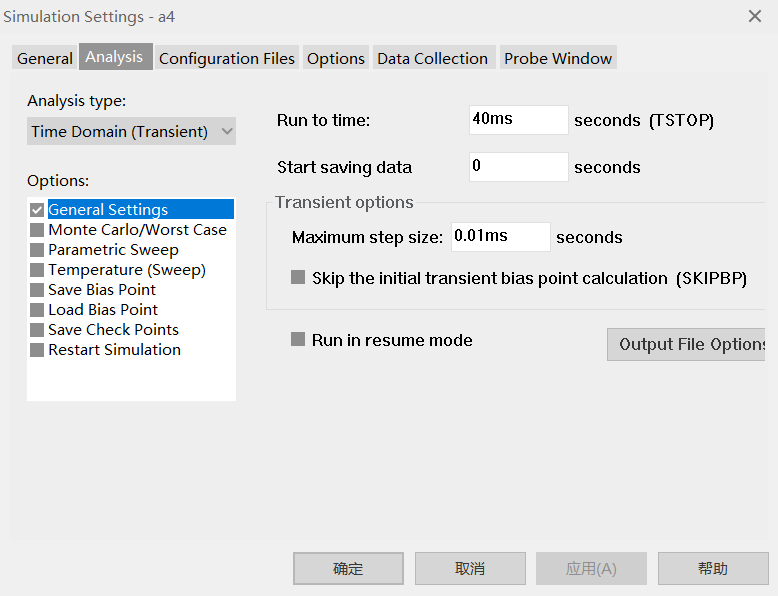
\includegraphics[scale = 0.6]{pic/桥式与稳压二极管/brg2.png}
                            \caption{桥式整流电路仿真分析设置参数}
                        \end{figure}
                        \item 进行仿真实验,分析波形。
                    \end{enumerate}
                \subsubsection{桥式整流电路分析}
                    \begin{enumerate}
                        \item 在OrCAD软件中按照图2连接好电路。
                        \item 根据电路电源的参数以及实验要求选择合适的仿真模式与参数。具体见下图。
                        \newpage
                        \begin{figure}[h]
                            \centering
                            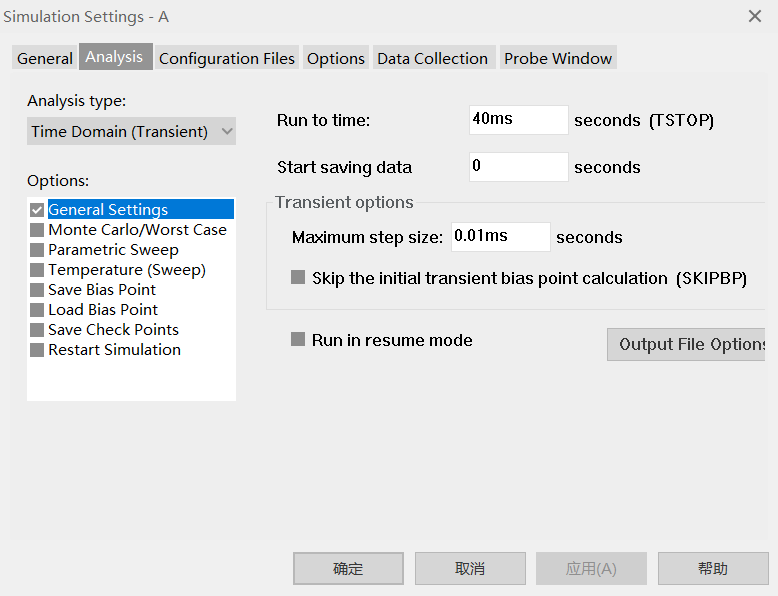
\includegraphics[scale = 0.6]{pic/桥式与稳压二极管/d2.png}
                            \caption{稳压二极管电路仿真分析设置参数}
                        \end{figure}
                        \item 进行仿真实验,分析波形。
                    \end{enumerate}
            \subsection{结果记录}
                \begin{figure}[h]
                    \centering
                    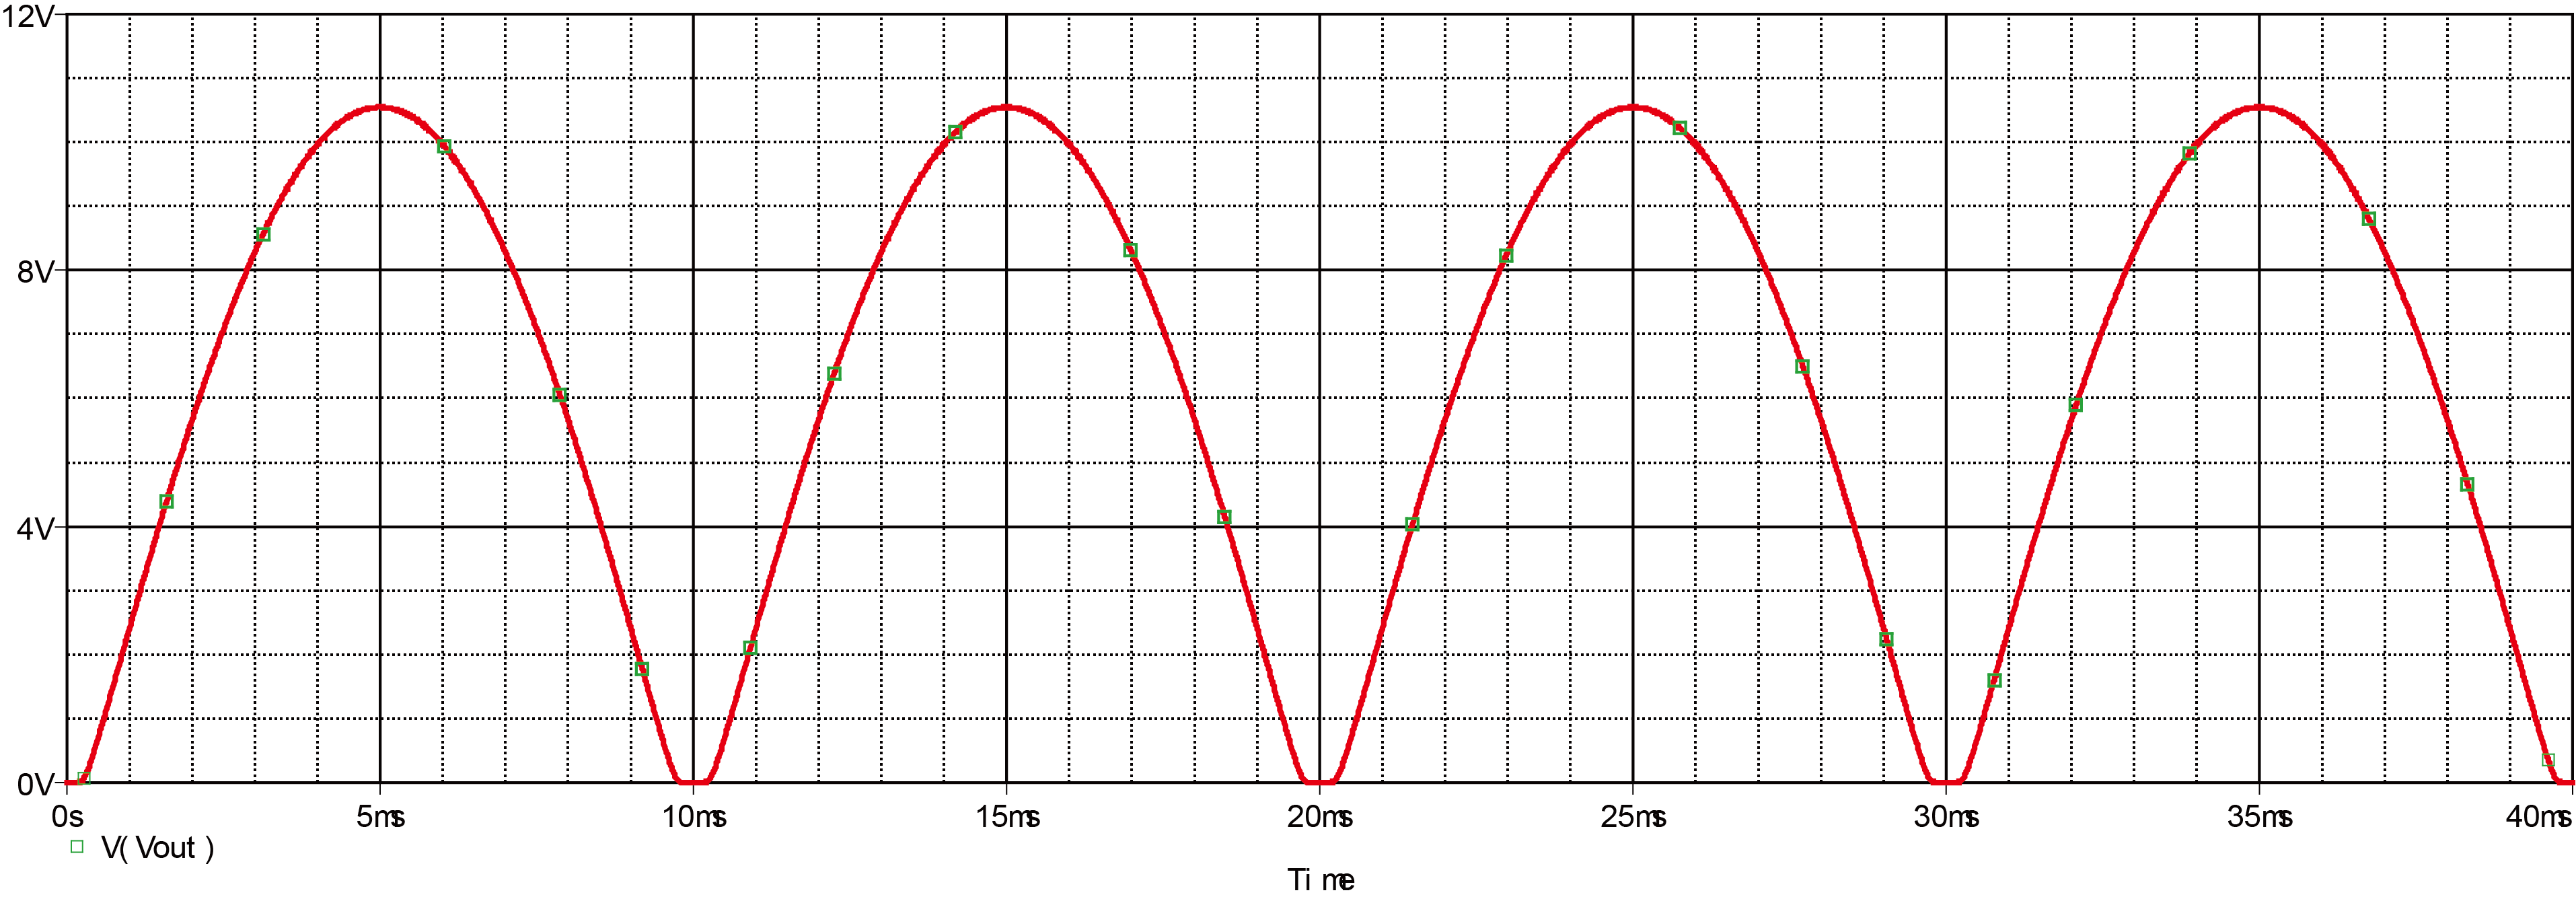
\includegraphics[scale=0.5]{pic/桥式与稳压二极管/brg3.png}
                    \caption{桥式整流电路仿真波形图}
                \end{figure}
                \newpage
                \begin{figure}[h]
                    \centering
                    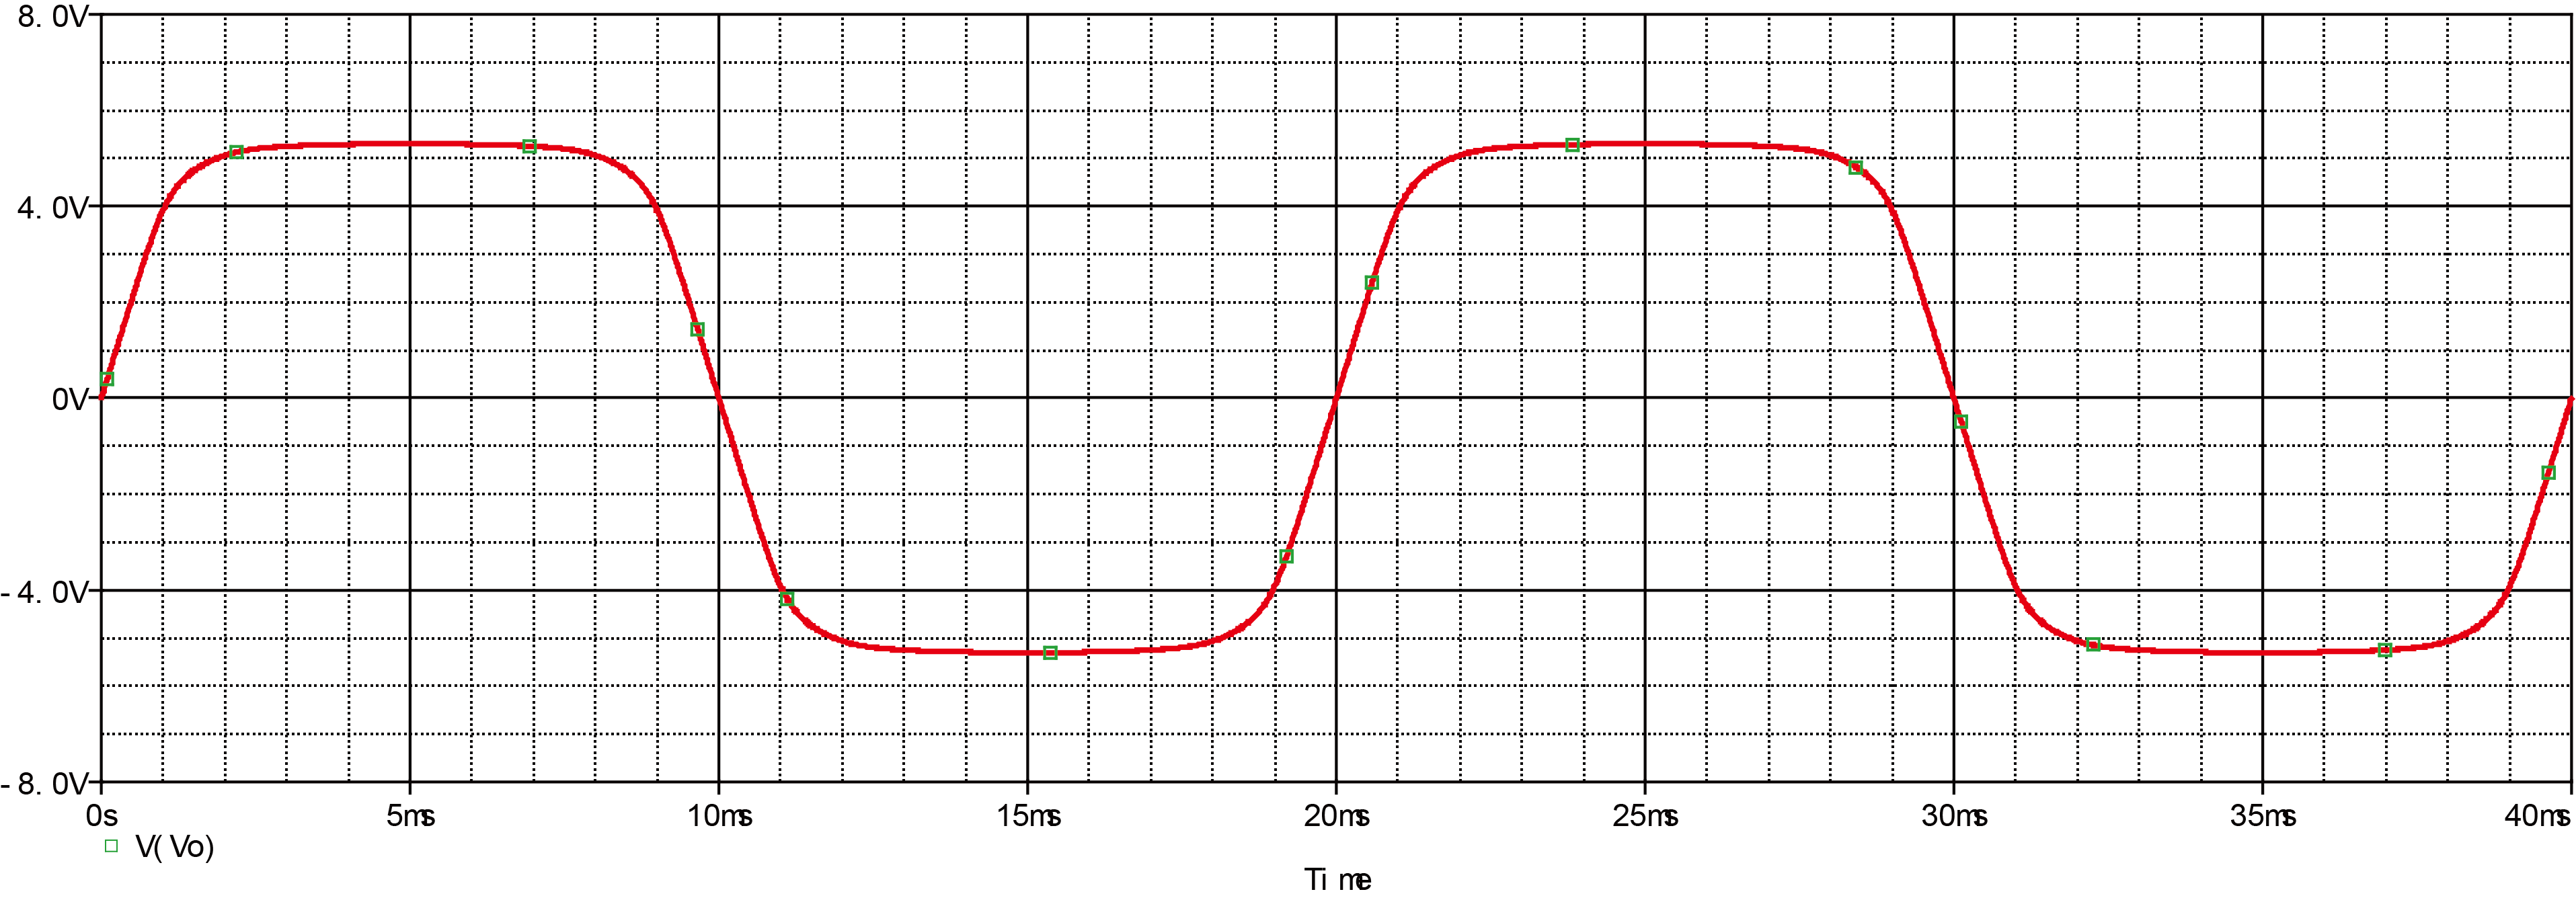
\includegraphics[scale=0.5]{pic/桥式与稳压二极管/d3.png}
                    \caption{稳压二极管电路仿真波形图}
                \end{figure}
    \section{实验结果和分析处理}
        \begin{enumerate}
            \item 由图5可以看出,经过桥式整流电路的整流,电阻$R$两端的输出电压只剩下正向电压,达到整流目的。
            \item 由图6可以看出,当我们电源电压选择$20V$时,稳压二极管两端的电压值超过了它的稳压值$4.7V$时,其输出波形产生了双向削顶现象,达到了稳压目的。
        \end{enumerate}
    \section{讨论、心得}
        通过本次实验,从对OrCAD软件的一无所知,变成了能熟练的应用该软件连接电路,并按照需求进行不同的仿真实验。
        通过本次实验,我也意识到利用软件进行仿真实验与实际实验相比的优越性。在利用软件仿真实验中,既提高了实验的效率,也节省了实验器材的成本。
        但是在实验的过程中我也遇到一些问题,在进行稳压二极管的输出波形分析时,最开始我的电源的电压时设置的$9V$,但是结果波形并没有出现双向削顶的现象,才意识到是稳压二极管的两端的电压并没有达到其稳压值,于是我讲电压源的电压上调到20V,这样以后就成功出现了双向削顶的现象。
    \section{思考题}
            \begin{enumerate}
                \item OrCAD软件在电路分析及设计过程中起什么作用?\par
                能够设计搭建电路,并对设计好的电路进行模拟仿真与分析。
                \item 用OrCAD软件对电路进行仿真分析时,是否要求每个节点必须有标号?在电路中设置节点标号有何作用?\par
                并不要求;在电路中设置节点标号可以让我们在仿真分析时更方便的找到节点。
                \item 用OrCAD的PSpice A/D中的Probe图形处理程序查看图形时,对于不同的分析设置,其缺省的横坐标是哪个变量?\par
                    \begin{enumerate}
                        \item 在时域分析中,缺省的横坐标是时间
                        \item 在直流分析中,缺省的是电源的电压值
                        \item 在交流分析中,缺省的是电源的频率
                        \item 在直流工作点分析中,是直接显示电路各个节点在直流工作点的电压值与支路的电流值,不会进行图像分析
                    \end{enumerate}
                \item 在仿真分析二极管特性测试电路的电压波形时,若瞬时分析不设置Maximum step size参数,则结果会出现什么情况?\par
                会出现信号失真,信号不再光滑。是因为当电源频率过大,系统默认的采样频率没有达到电源频率的两倍,不满足采样定理。
                \item 若要仿真分析三极管特性测试电路的输入特性,应如何设置扫描分析方式和参数?\par
                设置为直流扫描模式,纵坐标为$I_C$,X轴变量设置为三极管集电极与发射极之间的电压,选择合适的坐标范围。纵坐标为$I_C$.
            \end{enumerate}
\end{document}